\phantomsection
\part{集合}

\begin{abstract}
この章では，現代数学の基礎をなす「集合」を導入する．まず集合と元を定義し，集合の相等・部分集合・真部分集合といった基本概念を確認する．次に，$\mathbb{N}$，$\mathbb{Z}$，$\mathbb{Q}$，$\mathbb{R}$，$\mathbb{C}$ などのよく使う集合の記号と，外延的記法・内包的記法という集合の表記法を整理する．最後に，共通部分・和集合・差集合・補集合といった集合の演算を定義し，交換法則・分配律・ド・モルガンの法則などの基本性質を証明しよう．
\end{abstract}

\phantomsection
\section{集合の定義と表記法}

\phantomsection
\subsection{集合の定義}

現代数学の基礎をなす概念に「集合」や「写像」がある．まず「集合」からみていこう．
\phantomsection
\begin{definition}{集合}{集合}
  もののあつまりを\emph{集合}\index{しゅうごう@集合}という\footnote{公理的集合論の立場では，集合とは「無定義語」であるが，ここで詳しくは触れない．}．集合を構成するものを\emph{元}\index{げん@元}または\emph{要素}\index{ようそ@要素}といい，集合$A$の元が$a$であることを$a \in A$，$A \ni a$などと表す．
\end{definition}

\begin{remark}[集合の表記に関する注意]
  集合について，いくつか注意しておこう．
  \begin{itemize}
    \item 要素の順序は問わない．たとえば，$\{1,2,3\}=\{3,2,1\}$である．
    \item 同じ要素を重複して書いても同じ集合を表す．たとえば，$\{1,1,2,2,2,3\}=\{1,2,3\}$である．
    \item 異なる種類のものを要素にすることもできる．たとえば，$\{4,\{3\}\}$は数$4$と集合$\{3\}$を要素に持つ．
  \end{itemize}
\end{remark}

次に，ある集合の要素の一部または全部からなる集合を考える．これを\emph{部分集合}という．まずはその定義を確認し，具体例はのちほど紹介する．

\begin{definition}{集合の相等}{集合の相等}
  集合$A$，$B$のすべての要素が一致しているとき，$A$と$B$は\emph{相等}\index{そうとう@相等}であるといい，これを
  \[
    A = B
  \]
  と表す．

  また，集合$A$と$B$が相等でないとき，
  \[
    A \ne B
  \]
  と表す．
\end{definition}

\begin{remark}[相等を考える意義]
  \deref{集合の相等}を考える意義がぴんとこない読者もいるかもしれない．
  だが，たとえば$\pi$，$\int_{0}^{1} \frac{4}{1+x^2} \, dx$，$4 \sum_{n=0}^{\infty} \frac{(-1)^n}{2n+1}$は異なる表現であるが，すべて円周率を表している．
  このような例からわかるように，「相等」を考えることは数学的な主張を正確に表現するために重要なことなのだ．
\end{remark}

\phantomsection
\begin{definition}{部分集合}{部分集合}
  集合$A$の要素がすべて集合$B$の要素でもあるとき，$A$は$B$の\emph{部分集合}\index{ぶぶんしゅうごう@部分集合}であるといい，これを
  \[
    A \subset B,\quad B \supset A
  \]
  などと表す\footnote{このことを$ A \subseteq B$，$B \supseteq A$とかくこともある．一般に，$A \subset B$，$ B \supset A$と書いた場合には$A=B$の場合を含んで意味をとる．}．
\end{definition}

\begin{definition}{真部分集合}{真部分集合}
  集合$A$の要素がすべて集合$B$の要素であり，なおかつ$A \ne B$であるとき，$A$は$B$の\emph{真部分集合}\index{しんぶぶんしゅうごう@真部分集合}であるといい，これを
  \[
    A \subsetneq B,\quad B \supsetneq A
  \]
  などと表す．
\end{definition}

集合の相等は，部分集合の言葉を用いて次のように特徴づけられる．

\phantomsection
\begin{prop}{相等と相互包含}{相等と相互包含}
  集合$A$，$B$に対して，
  \[
    A = B
    \lequiv
    (A \subset B) \land (B \subset A)
  \]
  である．また，量化子を用いれば，
  \[
    A = B
    \lequiv
    \lall{x} \lst ( x \in A \lequiv x \in B )
  \]
  と表すこともできる．
\end{prop}

\begin{tleftbar}
  \begin{proof}
    \deref{集合の相等}より，$A = B$とは$A$と$B$のすべての要素が一致すること，すなわち「任意の$x$について，$x \in A$と$x \in B$の真偽が一致する」ことである．一方，$A \subset B$は「任意の$x$について，$x \in A$ならば$x \in B$」を，$B \subset A$は「任意の$x$について，$x \in B$ならば$x \in A$」を意味する．同値の等価表現$P \lequiv Q \equiv (P \limp Q) \land (Q \limp P)$により，両者は一致する．これが証明すべきことであった．
  \end{proof}
\end{tleftbar}

この命題は，集合の等式$A = B$を証明するための\textbf{標準的な方法}を与えている．すなわち，$A \subset B$と$B \subset A$の\textbf{両方向の包含}をそれぞれ示せばよい．のちに集合の分配律を証明する際にも，実際にこの方法を用いる．

\phantomsection
\subsection{集合の表記}

集合を表す方法には，おもに次の2つがある．

\begin{description}
  \item[外延的記法\index{がいえんてききほう@外延的記法}（列挙形式）]
        $\{a,b,c\}$のように，要素を列挙して表す．
  \item[内包的記法\index{ないほうてききほう@内包的記法}（条件形式）]
        $\{x\in\mathbb{N}\mid x\leqq5\}$のように，
        要素が満たす条件を用いて表す．
\end{description}

\begin{example}{集合の表記}{集合の表記}
  集合は，外延的記法と内包的記法のどちらを用いても表すことができる．
  たとえば，次の等式が成り立つ．
  \begin{align*}
    \{1,2,3\}
      &=
      \{n\in\mathbb{N}\mid n^2-4n+3\leqq0\},\\
    \{-2,-1,0,1,2\}
      &=
      \{n\in\mathbb{Z}\mid n^2\leqq4\},\\
    \{2,4,6,8,\dots\}
      &=
      \{2n\mid n\in\mathbb{N}\},\\
    \{1,4,9,16,25,\dots\}
      &=
      \{n^2\mid n\in\mathbb{N}\},\\
      \{-1,1\} &= \{x\in\mathbb{R}\mid x^{2026}=1\}.
  \end{align*}
\end{example}

また数学では，よく使われる集合に固有の記号を用いることがある．

\begin{reviewbox}[数の集合]
  \small
  \begin{tabular}{@{}p{14\zw}@{\hspace{1.5\zw}}l@{}}
    自然数（natural numbers）&
    $\mathbb{N} = \{1,2,3,\ldots\}$\footnotemark\\[0.35\baselineskip]

    整数（integers）&
    $\mathbb{Z} = \{\ldots,-2,-1,0,1,2,\ldots\}$\\[0.35\baselineskip]

    有理数（rational numbers）&
    $\mathbb{Q} = \left\{ \frac{a}{b} \relmiddle| a \in \mathbb{Z},\ b \in \mathbb{N} \right\}$\\[0.35\baselineskip]

    実数（real numbers）&
    $\mathbb{R}$\\[0.35\baselineskip]

    複素数（complex numbers）&
    $\mathbb{C} = \{ a + bi \mid a,b \in \mathbb{R} \}$
  \end{tabular}
  \footnotetext{自然数に$0$を含める流儀もあるが，本書では自然数に$0$を含めないものとする．}
\end{reviewbox}

$\mathbb{N}$，$\mathbb{R}$，$\mathbb{C}$は，それぞれ natural number，real number，complex number に由来する記号である．
また，$\mathbb{Z}$はドイツ語の Zahl（数）に，$\mathbb{Q}$は quotient（商）に由来する．
なお，$\mathbb{C}$の表記に現れる$i$は，$i^2 = -1$を満たす\emph{虚数単位}である．$i$は内包的記法の中で動く変数ではなく，あらかじめ固定された定数であることに注意したい．


$x$がどの集合の中を動くかは，文脈により省略されることがある．たとえば，以下のような問題があったとする．
\begin{quotation}
  方程式
  \[
    x^2 + 1 = 0
  \]
  を解け．
\end{quotation}
この問題では，$x$がどの集合の中を動くかが明記されていない．
もし$x \in \mathbb{R}$の範囲で解を探すなら，任意の実数$x$に対して$x^2 + 1 \geqq 1 > 0$なので，解は存在しない．
一方，$x \in \mathbb{C}$の範囲で解を探すなら，解は$x = \pm i$である．
このように，「方程式を解く」という問題の答えは，\textbf{どの集合の中で解を探しているか}によって変わる．
$x$が動く集合は，文脈から読み取れたり明記されていたりする場合が多いが，答えが変わりうる以上，つねに意識しておきたいことがらである．

数の集合以外にも，特定の集合を表すために固有の記号を用いることがある．

\phantomsection
\begin{definition}{空集合}{空集合}
  要素をひとつも持たない集合を\emph{空集合}\index{くうしゅうごう@空集合}といい，
  \[
    \varnothing
  \]
  で表す．
\end{definition}

空集合は$\emptyset$と表記することもある\footnote{空集合をギリシャ文字の$\phi$で表記するのは誤りである．空集合の記号$\varnothing$はAndré Weilによって導入されたもので，ノルウェー語やデンマーク語などで用いられる文字Øに着想を得ている．}．

\phantomsection
\begin{example}{空集合の例}{空集合の例}
  空集合は，外延的記法では
  \[
    \{\}
  \]
  と表される．一方，内包的記法では，たとえば
  \[
    \{x \in \mathbb{R} \mid x^2=-1\},
    \qquad
    \{n \in \mathbb{N} \mid n<0\},
    \qquad
    \{x \in \mathbb{R} \mid x<x\}
  \]
  は，いずれも条件を満たす要素をひとつも持たないため，空集合である．
  したがって，
  \[
    \{\}
    =
    \{x \in \mathbb{R} \mid x^2=-1\}
    =
    \{n \in \mathbb{N} \mid n<0\}
    =
    \{x \in \mathbb{R} \mid x<x\}
    =
    \varnothing
  \]
  である．
\end{example}

\begin{remark}[空集合に関する注意]
  空集合について，いくつか注意しておこう．
  \begin{itemize}
    \item 空集合は要素をひとつも持たないので，どのような$x$に対しても，$x \in \varnothing$は\textbf{常に偽}である．いいかえれば，任意の$x$に対して$x \notin \varnothing$が成り立つ．
    \item 集合
          \[
            \{\varnothing\}
          \]
          は空集合$\varnothing$をひとつの要素として持つ集合であり，空集合ではない．
    \item 空集合の要素の個数は$0$である．一般に，有限集合$A$の要素の個数を$|A|$や$n(A)$と表すことがあり，この記法を用いれば
          \[
            |\varnothing| = 0, \qquad |\{\varnothing\}| = 1
          \]
          である．
  \end{itemize}
\end{remark}

\phantomsection
\begin{example}{所属関係の例}{所属関係の例}
  \[
    x \in \mathbb{Q}
  \]
  とかくことで，$x$は有理数であることを表す．
\end{example}

\phantomsection
\begin{example}{部分集合の例}{部分集合の例}
  \[
    \mathbb{R} \subset \mathbb{C}
  \]
  である．つまり，実数全体の集合は複素数全体の集合の部分集合である．
\end{example}

\phantomsection
\begin{prop}{空集合は任意の集合の部分集合}{空集合は任意の集合の部分集合}
  $A$を任意の集合とするとき，
  \[
    \varnothing \subset A
  \]
  である．つまり，空集合はすべての集合の部分集合である．
\end{prop}

\begin{tleftbar}
  \begin{proof}
    部分集合の定義（\deref{部分集合}）より，$\varnothing \subset A$を示すには，
    \begin{quotation}
      任意の$x$に対して，$x \in \varnothing$ならば$x \in A$である
    \end{quotation}
    ことを示せばよい．ところが，空集合は要素をひとつも持たないので，$x \in \varnothing$を満たす$x$は存在しない．すなわち，仮定「$x \in \varnothing$」はどのような$x$に対しても偽である．仮定が偽である命題は結論によらず真であるから\footnote{このように，仮定を満たすものが存在しないために無条件で真となることを，\emph{空虚な真}（vacuous truth）ということがある．}，「$x \in \varnothing$ならば$x \in A$」は任意の$x$に対して真である．よって$\varnothing \subset A$が成り立つ．
  \end{proof}
\end{tleftbar}

\begin{remark}[背理法による見方]
  次のように考えることもできる．もし$\varnothing \subset A$が成り立たないとすると，「$\varnothing$の要素であって$A$に属さないもの」が少なくともひとつ存在しなければならない．しかし，$\varnothing$はそもそも要素を持たないので，そのような要素は存在しえない．よって$\varnothing \subset A$である．
\end{remark}

集合を要素とする集合の重要な例として，べき集合がある．

\phantomsection
\begin{definition}{べき集合}{べき集合}
  集合$A$に対して，$A$の部分集合全体からなる集合
  \[
    \mathcal{P}(A) \coloneqq \{ B \mid B \subset A \}
  \]
  を$A$の\emph{べき集合}\index{べきしゅうごう@べき集合}という．
\end{definition}

\prref{空集合は任意の集合の部分集合}により，つねに$\varnothing \in \mathcal{P}(A)$である．また，$A \subset A$なので$A \in \mathcal{P}(A)$である．

\phantomsection
\begin{example}{べき集合}{べき集合}
  $A=\{ 1, 2\}$とすると，
  \[
    \mathcal{P}(A) = \{ \varnothing, \{1\}, \{2\}, \{1, 2\}\}
  \]
  である．
\end{example}



\phantomsection
\section{集合の演算}

\subsection{共通部分・和集合・差集合・補集合}
集合に対して，以下のような演算を定義することができる．

\phantomsection
\begin{definition}{共通部分・和集合・差集合・補集合}{共通部分・和集合・差集合・補集合}
  $A$と$B$を集合とするとき，以下の定義をする．
  \begin{description}
    \item[共通部分\index{きょうつうぶぶん@共通部分}]\mbox{}\\
          $A$と$B$の両方に属する要素全体の集合を$A \cap B$と表す．これを``$A$ intersection $B$''と読む．
    \item[和集合\index{わしゅうごう@和集合}]\mbox{}\\
          $A$または$B$のいずれかに属する要素全体の集合を$A \cup B$と表す．これを``$A$ union $B$''と読む．
    \item[差集合\index{さしゅうごう@差集合}]\mbox{}\\
          $A$の要素で$B$に属さないもの全体の集合を$A \setminus B$と表す．
    \item[補集合\index{ほしゅうごう@補集合}]\mbox{}\\
          全体集合$X$\footnote{考察の対象すべてを含む集合をあらかじめひとつ固定して考えるとき，その集合を\emph{全体集合}\index{ぜんたいしゅうごう@全体集合}という．}とその部分集合$A \subset X$に対して，$A^c \coloneqq X \setminus A$を$A$の補集合という．これを``$A$ complement''と読む．
  \end{description}
\end{definition}

\begin{remark}[論理記号による言い換え]
  集合の演算は，\partref{論理}で学んだ論理記号を用いて次のように言い換えられる：
  \begin{align*}
    x \in A \cap B & \lequiv (x \in A) \land (x \in B), \\
    x \in A \cup B & \lequiv (x \in A) \lor (x \in B), \\
    x \in A \setminus B & \lequiv (x \in A) \land \lnot (x \in B), \\
    x \in A^c & \lequiv \lnot (x \in A) \qquad (x \in X)
  \end{align*}
  すなわち，$\cap$は$\land$に，$\cup$は$\lor$に，補集合は$\lnot$に対応している．また，部分集合についても
  \[
    A \subset B \lequiv \lall{x} \lst ( x \in A \limp x \in B )
  \]
  である．この対応により，命題論理の法則から集合の法則を導くことができる（のちのド・モルガンの法則の証明で実際に用いる）．
\end{remark}


\begin{figure}[ht]
  \centering
  % --- ベン図の共通設定 ---
  \tikzset{
    venn frame/.style={
      draw=black!75,
      line width=0.7pt
    },
    venn circle/.style={
      draw=black!85,
      line width=0.8pt
    },
    venn fill/.style={
      fill=magenta!15
    },
    venn label/.style={
      font=\small
    }
  }
  % --- 共通部分 ---
  \begin{minipage}{0.45\linewidth}
    \centering
    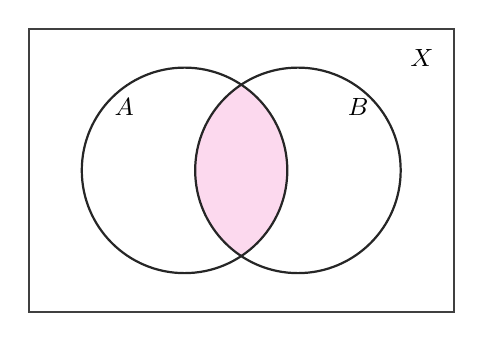
\begin{tikzpicture}[scale=0.9]
      % 塗り
      \begin{scope}
        \clip (2.2,2) circle (1.45);
        \fill[venn fill] (3.8,2) circle (1.45);
      \end{scope}

      % 輪郭
      \draw[venn frame] (0,0) rectangle (6,4);
      \draw[venn circle] (2.2,2) circle (1.45);
      \draw[venn circle] (3.8,2) circle (1.45);

      % ラベル
      \node[venn label] at (1.35,2.9) {$A$};
      \node[venn label] at (4.65,2.9) {$B$};
      \node[venn label, anchor=north east] at (5.85,3.85) {$X$};
    \end{tikzpicture}
    \caption{共通部分 $A \cap B$}
  \end{minipage}
  \hfill
  % --- 和集合 ---
  \begin{minipage}{0.45\linewidth}
    \centering
    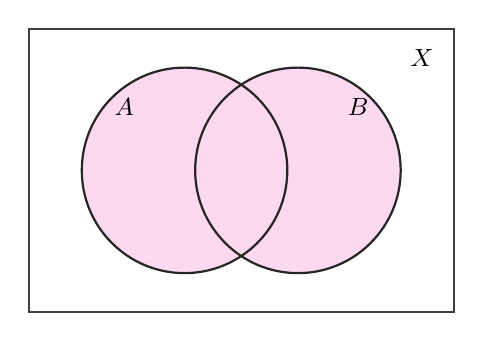
\begin{tikzpicture}[scale=0.9]
      % 塗り
      \fill[venn fill] (2.2,2) circle (1.45);
      \fill[venn fill] (3.8,2) circle (1.45);

      % 輪郭
      \draw[venn frame] (0,0) rectangle (6,4);
      \draw[venn circle] (2.2,2) circle (1.45);
      \draw[venn circle] (3.8,2) circle (1.45);

      % ラベル
      \node[venn label] at (1.35,2.9) {$A$};
      \node[venn label] at (4.65,2.9) {$B$};
      \node[venn label, anchor=north east] at (5.85,3.85) {$X$};
    \end{tikzpicture}
    \caption{和集合 $A \cup B$}
  \end{minipage}

  \vspace{3mm}

  % --- 差集合 ---
  \begin{minipage}{0.45\linewidth}
    \centering
    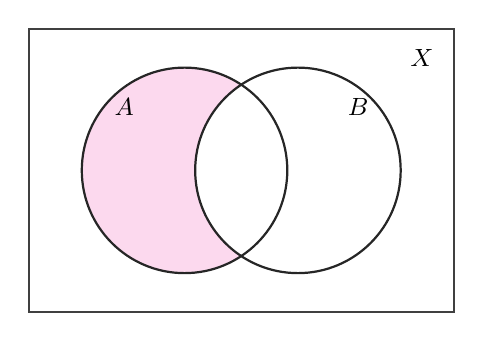
\begin{tikzpicture}[scale=0.9]
      % A を塗る
      \fill[venn fill] (2.2,2) circle (1.45);

      % A \cap B の部分を白く戻す
      \begin{scope}
        \clip (2.2,2) circle (1.45);
        \fill[white] (3.8,2) circle (1.45);
      \end{scope}

      % 輪郭
      \draw[venn frame] (0,0) rectangle (6,4);
      \draw[venn circle] (2.2,2) circle (1.45);
      \draw[venn circle] (3.8,2) circle (1.45);

      % ラベル
      \node[venn label] at (1.35,2.9) {$A$};
      \node[venn label] at (4.65,2.9) {$B$};
      \node[venn label, anchor=north east] at (5.85,3.85) {$X$};
    \end{tikzpicture}
    \caption{差集合 $A \setminus B$}
  \end{minipage}
  \hfill
  % --- 補集合 ---
  \begin{minipage}{0.45\linewidth}
    \centering
    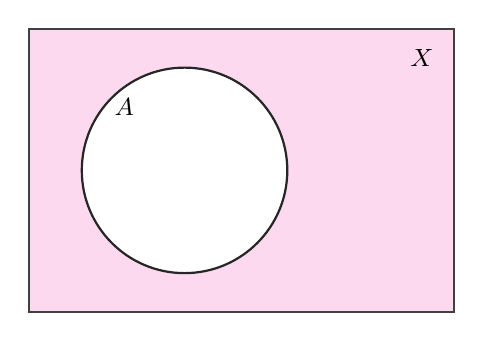
\begin{tikzpicture}[scale=0.9]
      % X 全体を塗る
      \fill[venn fill] (0,0) rectangle (6,4);

      % A を白く抜く
      \fill[white] (2.2,2) circle (1.45);

      % 輪郭
      \draw[venn frame] (0,0) rectangle (6,4);
      \draw[venn circle] (2.2,2) circle (1.45);

      % ラベル
      \node[venn label] at (1.35,2.9) {$A$};
      \node[venn label, anchor=north east] at (5.85,3.85) {$X$};
    \end{tikzpicture}
    \caption{補集合 $A^c$}
  \end{minipage}
\end{figure}


\phantomsection
\begin{example}{集合}{集合}
  たとえば，$A = \{1, 2, 3\}$，$B = \{3, 4, 5\}$とすると，
  \begin{itemize*}
    \item $A \cap B = \{3\}$
    \item $A \cup B = \{1, 2, 3, 4, 5\}$
    \item $A \setminus B = \{1, 2\}$
    \item $X=\{1,2,3,4,5\}$とすると，$A^c = \{4, 5\}$
  \end{itemize*}
\end{example}

\begin{prop}{集合の交換法則}{集合の交換法則}
  $A$，$B$を集合とするとき，
  \[
    A \cap B = B \cap A , \quad A \cup B = B \cup A
  \]
  である．
\end{prop}

\begin{tleftbar}
  \begin{proof}
    共通部分および和集合の定義から従う．
  \end{proof}
\end{tleftbar}

\begin{remark}[交換法則を考える意義]
  ここで「なぜ交換法則を考えるのか」という疑問が生じるかもしれない．当たり前に成り立つことだと思える読者もいるかもしれないが，よく考えてみると「実数の減法」や「関数（写像）の合成」，「行列の積」など，
  数学において一般に交換法則が成り立たないものは数多く存在する．集合に対して交換法則を考える意義はそこにあるのである．
\end{remark}

\phantomsection
\begin{prop}{空集合との演算}{空集合との演算}
  $A$を任意の集合とするとき，
  \[
    A \cup \varnothing = A, \quad A \cap \varnothing = \varnothing
  \]
  である．
\end{prop}

\begin{tleftbar}
  \begin{proof}
    まず$A \cup \varnothing = A$を示す．$x \in A \cup \varnothing$とすると，$x \in A$または$x \in \varnothing$である．$x \in \varnothing$を満たす$x$は存在しないので，$x \in A$でなければならない．よって$A \cup \varnothing \subset A$である．逆に，$x \in A$ならば和集合の定義から$x \in A \cup \varnothing$なので，$A \subset A \cup \varnothing$である．以上より$A \cup \varnothing = A$が成り立つ．

    次に$A \cap \varnothing = \varnothing$を示す．$x \in A \cap \varnothing$とすると，特に$x \in \varnothing$であるが，そのような$x$は存在しない．すなわち$A \cap \varnothing$は要素をひとつも持たないので，$A \cap \varnothing = \varnothing$である．
  \end{proof}
\end{tleftbar}

\begin{remark}[空集合と差集合・直積]
  差集合についても，
  \[
    A \setminus \varnothing = A, \quad \varnothing \setminus A = \varnothing
  \]
  が成り立つ．これは差集合の定義から直ちに確かめられる．

  また，集合$A$，$B$に対して，$A$の要素と$B$の要素の順序対$(a,b)$全体の集合を\emph{直積}$A \times B$という（詳しくは\partref{写像}で定義する）．直積についても，
  \[
    A \times \varnothing = \varnothing, \quad \varnothing \times A = \varnothing
  \]
  が成り立つ．たとえば$(a, b) \in A \times \varnothing$となる順序対が存在するとすれば，$b \in \varnothing$でなければならないが，そのような$b$は存在しないからである．
\end{remark}

\subsection{集合の分配律}

\phantomsection
\begin{prop}{集合の分配律}{集合の分配律}
  $A$，$B$，$C$を集合とするとき，
  \begin{align*}
    A \cap ( B \cup C) & = (A \cap B) \cup (A \cap C), \\
    A \cup ( B \cap C) & = (A \cup B) \cap (A \cup C)
  \end{align*}
\end{prop}

\begin{tleftbar}
  \begin{proof}
    まず，
    \[
      A \cap (B \cup C) \subset (A \cap B) \cup (A \cap C)
    \]
    を示す：

    $x \in A \cap (B \cup C)$ とすると，$x$ は $A$ に属し，かつ $B \cup C$ に属する．
    すると $x \in B \cup C$ なので，$x \in B$ または $x \in C$ のいずれかが成り立つ．
    \begin{itemize}
      \item もし $x \in B$ であれば，$x$ は $A$ に属し $B$ にも属するので，$x \in A \cap B$ となる．よって $x \in (A \cap B) \cup (A \cap C)$ が従う．
      \item もし $x \in C$ であれば，$x$ は $A$ に属し $C$ にも属するので，$x \in A \cap C$ となる．よって $x \in (A \cap B) \cup (A \cap C)$ が従う．
    \end{itemize}
    いずれの場合でも $x \in (A \cap B) \cup (A \cap C)$ となるので，
    \[
      A \cap (B \cup C) \subset (A \cap B) \cup (A \cap C)
    \]
    が示された．

    次に，
    \[
      (A \cap B) \cup (A \cap C) \subset A \cap (B \cup C)
    \]
    を示す：

    $x \in (A \cap B) \cup (A \cap C)$ とすると，$x \in A \cap B$ または $x \in A \cap C$ のいずれかが成り立つ．
    \begin{itemize}
      \item もし $x \in A \cap B$ であれば，$x$ は $A$ に属し，かつ $B$ に属する．すると $B \subset B \cup C$ だから $x \in B \cup C$ でもある．よって $x \in A \cap (B \cup C)$ が成り立つ．
      \item もし $x \in A \cap C$ であれば，$x$ は $A$ に属し，かつ $C$ に属する．すると $C \subset B \cup C$ だから $x \in B \cup C$ でもある．よって $x \in A \cap (B \cup C)$ が成り立つ．
    \end{itemize}
    いずれの場合でも $x \in A \cap (B \cup C)$ となるので，
    \[
      (A \cap B) \cup (A \cap C) \subset A \cap (B \cup C)
    \]
    が示された．

    以上の2つの包含関係から，
    \[
      A \cap (B \cup C) =(A \cap B) \cup (A \cap C)
    \]
    が成り立つ．後半の等式も同様に示される．これが証明すべきことであった．
  \end{proof}
\end{tleftbar}

\subsection{集合のさまざまな法則}

\phantomsection
\begin{prop}{べき等律・全体集合との演算・補集合の性質}{べき等律・全体集合との演算・補集合の性質}
  $X$を全体集合，$A \subset X$とするとき，次が成り立つ：
  \begin{align*}
    & A \cup A = A, && A \cap A = A, \\
    & A \cup X = X, && A \cap X = A, \\
    & A \cup A^c = X, && A \cap A^c = \varnothing, \\
    & (A^c)^c = A
  \end{align*}
\end{prop}

\begin{tleftbar}
  \begin{proof}
    いずれも定義から確かめられる．例として$(A^c)^c = A$を示す．$x \in X$に対して，
    \[
      x \in (A^c)^c
      \lequiv \lnot ( x \in A^c )
      \lequiv \lnot \lnot ( x \in A )
      \lequiv x \in A
    \]
    である（最後の同値は二重否定$\lnot \lnot P \equiv P$による）．よって$(A^c)^c = A$である．残りも同様に示される．
  \end{proof}
\end{tleftbar}

\phantomsection
\begin{prop}{集合のド・モルガンの法則}{集合のド・モルガンの法則}
  $X$を全体集合，$A, B \subset X$とするとき，
  \[
    (A \cup B)^c = A^c \cap B^c,
    \qquad
    (A \cap B)^c = A^c \cup B^c
  \]
  が成り立つ．
\end{prop}

\begin{tleftbar}
  \begin{proof}
    前半を示す．$x \in X$に対して，
    \begin{align*}
      x \in (A \cup B)^c
      & \lequiv \lnot ( x \in A \cup B ) \\
      & \lequiv \lnot \bigl( (x \in A) \lor (x \in B) \bigr) \\
      & \lequiv \lnot (x \in A) \land \lnot (x \in B) \\
      & \lequiv x \in A^c \cap B^c
    \end{align*}
    である．途中，3つ目の同値で命題論理のド・モルガンの法則$\lnot (P \lor Q) \equiv \lnot P \land \lnot Q$を用いた．\prref{相等と相互包含}の論理式による特徴づけにより，$(A \cup B)^c = A^c \cap B^c$である．後半も同様に示される．これが証明すべきことであった．
  \end{proof}
\end{tleftbar}

\begin{remark}[論理の法則と集合の法則]
  この証明からわかるように，集合のド・モルガンの法則は，命題論理のド・モルガンの法則を$P = (x \in A)$，$Q = (x \in B)$として集合の言葉に翻訳したものにほかならない．同様に，集合の交換法則・結合律・分配律も，命題論理の対応する法則から導くことができる．論理と集合は，このように同じ構造を共有しているのである．
\end{remark}
% NOTE: この部は執筆中（今後，節を追記する可能性あり）
